\chapter{Introduction}\label{introduction}

% Social media has become an essential part of modern life, enabling billions of people to share their stories, connect over shared interests, and participate in discussions on global events. This has resulted in the formation of large online communities. Unlike physical communities, online communities allow for easier and more immediate grouping of individuals, as joining a community often requires minimal effort; simply clicking a button or following a page \cite{ellison:2007}. This ease of access fosters the creation of diverse and dynamic social ecosystems, where users interact under shared norms, behaviors, and communication styles unique to each community.

% However, the aggregation of large numbers of individuals in online communities also increases the likelihood of negative behaviors, such as toxicity. Toxicity in online spaces refers to harmful actions, including hate speech, racism, sexism, and other forms of discrimination \cite{fan:2022}. These behaviors are often exacerbated by the anonymity and reduced social inhibitions that characterize digital environments \cite{suler:2004,moore:2012,wulczyn:2016}.

Social media platforms reinforce the risk of toxic behavior, such as hate speech, harassment, and discrimination, compared to traditional media, due to their scale, anonymity, and minimal barriers to community entry \cite{fan:2022,suler:2004,ellison:2007}. While these platforms enable billions to connect and share opinions, their design encourages environments where harmful actions thrive. For instance, the ease of joining online communities (often just a click away) encourages rapid aggregation of users \cite{ellison:2007} but also decreases the sense of responsibility, as anonymity reduces social inhibitions \cite{moore:2012,suler:2004,wulczyn:2017}. This dynamic creates fertile ground for toxicity, which spreads easier in digital spaces than in physical interactions \cite{suler:2004}.

\begin{figure}[tb]
  \centering
  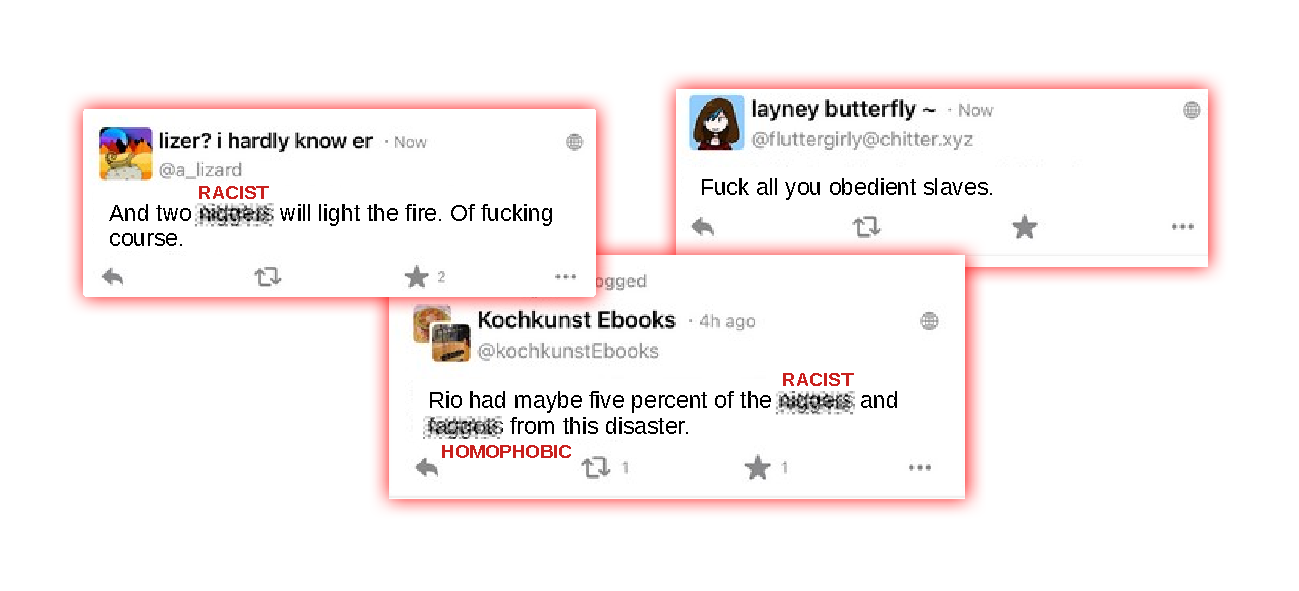
\includegraphics[width=\linewidth]{../material/toxic_comments.pdf}
  \caption{Three toxic examples posted during the 2024 Paris Olympics opening ceremony on Mastodon. The toots shown here contain real content but have been recreated and do not show the real user.}
  \label{toxic-comments}
\end{figure}

Behaviors, like those you can see in Figure\ref{toxic-comments} disrupt community solidarity and harm individual users, making toxicity a significant challenge for social media platforms \cite{fan:2022,wulczyn:2017}. To mitigate these issues, online communities establish rules and moderation systems to enforce acceptable behavior. Violations of these rules can result in penalties, such as bans or restrictions, depending on the platform's moderation policies \cite{nicholson:2023}.

\begin{figure}[tb]
  \centering
  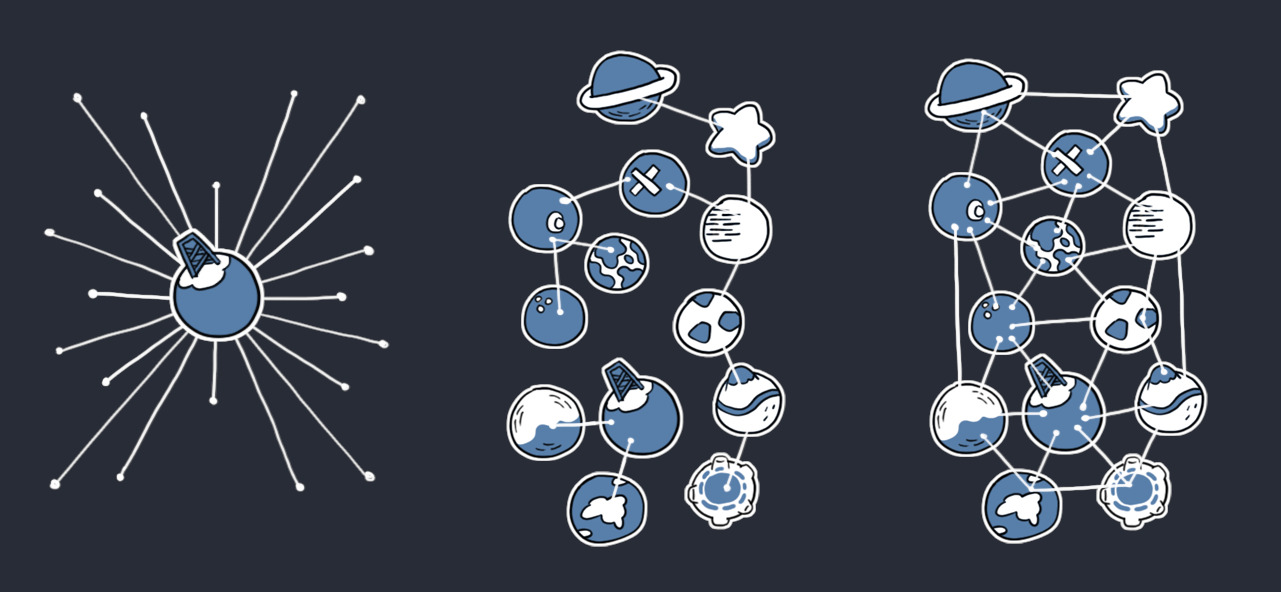
\includegraphics[width=\textwidth]{../material/network_models.jpg}
  \caption{From left to right: Centralized networks connect all through a single controlling hub; Federated networks organize nodes into semi-autonomous interconnected clusters; Distributed networks connect all nodes with multiple pathways \cite{mastodon:docs}.}
  \label{network-models}
\end{figure}

To understand the dynamics of toxicity in online communities and the challenges they face, this case study focuses on Mastodon\footnote{\url{https://mastodon.social/explore}}, a decentralized alternative to traditional social media platforms like Twitter/X\footnote{\url{https://x.com/}}. The recent acquisition of Twitter/X by Elon Musk has highlighted the risks of centralized social media, where a single individual or entity can exert significant control over platform governance, content moderation, and user experience \cite{he:2023}. Such centralization can lead to abrupt policy changes, increased misinformation, and heightened toxicity, prompting users to seek alternatives. Mastodon, as a decentralized and federated platform, offers a contrasting model where power is distributed across independently operated instances. In common with other social media platforms, Mastodon offers the possibility to interact with other people by publishing posts, reacting to posts, or sharing posts. However, Mastodon as a federated social media platform belongs to the decentralized online social networks (DOSNs). Federation refers to a special kind of decentralization explained in Figure~\ref{network-models}. Traditional social media platforms, such as Twitter/X, Facebook, or Instagram, have a single central service that all users access. In contrast, Mastodon has multiple services, called instances, which are used by any number of people. These instances can communicate with each other and create a federated network. Users can freely choose an instance based on language, community rules, moderation policies, and topics of interest. Each instance is managed by its own administrators, who set and enforce local rules \cite{mastodon:docs}. However, this decentralization also introduces unique challenges, such as inconsistent moderation standards and the potential for fragmentation within the fediverse \cite{he:2023}. By examining Mastodon, this study aims to explore how decentralized platforms address toxicity and community management while navigating the complexities of a federated ecosystem.

\paragraph{Research Gap and Contribution}
Prior work has established foundational knowledge about Mastodon's structure \cite{zulli:2020,la_cava:2021}, moderation practices \cite{bono:2024,nicholson:2023}, and toxicity analysis methods \cite{fan:2022}. However, only a few studies have systematically examined toxicity patterns across the entire Mastodon network and those are limited on small datasets, such as the study by \citet{al-khateeb:2022}. Our research addresses this gap by conducting a large-scale toxicity analysis of Mastodon. We analyzed a 1\% subsample of 1.8~billion Mastodon posts (called ``toots'') across 1,000~instances collected throughout 2024. The results reveal two key findings: First, toxicity levels show clear spikes during major political and global events, particularly around the U.S.~election period. Second, active moderation practices seem to lower mean toxicity levels on instances, demonstrating the effectiveness of decentralized moderation approaches.

\enlargethispage{\baselineskip}